\documentclass{article}
\usepackage[utf8]{inputenc}
\usepackage{geometry}
\usepackage{graphicx}
\usepackage{pgfplots}
\usepackage{verbatim}
\usepackage{amssymb}
\usepackage{amsmath}

\geometry{a4paper, left=2cm, right=2cm, top=1cm, bottom=2cm}

\begin{document}

\begin{minipage}{0.7\textwidth}
    \small \textbf{MECÁNICA VECTORIAL}  \\
    \small {Facultad de Ciencias, Universidad Nacional Autónoma de México} \\
    \small {Fecha de entrega: 16 de Febrero de 2023} \\
    \small {Nombre completo: Andrés López González} \\
    \small {Tarea número 2}
\end{minipage}
\hfill
\begin{minipage}{0.12\textwidth}
    
\includegraphics[width=\linewidth]{logo_universidad}
\end{minipage}

\section*{Tarea segunda semana}

XXI. Para cada una de las situaciones siguientes, trace una gráfica que sea una descripción posible de la posición en función del tiempo de una partícula que se mueve a lo largo del eje x. En t = 1 s, la partícula tiene\\
(a) velocidad cero y aceleración positiva;\\
\begin{figure}[htbp]
    \centering
    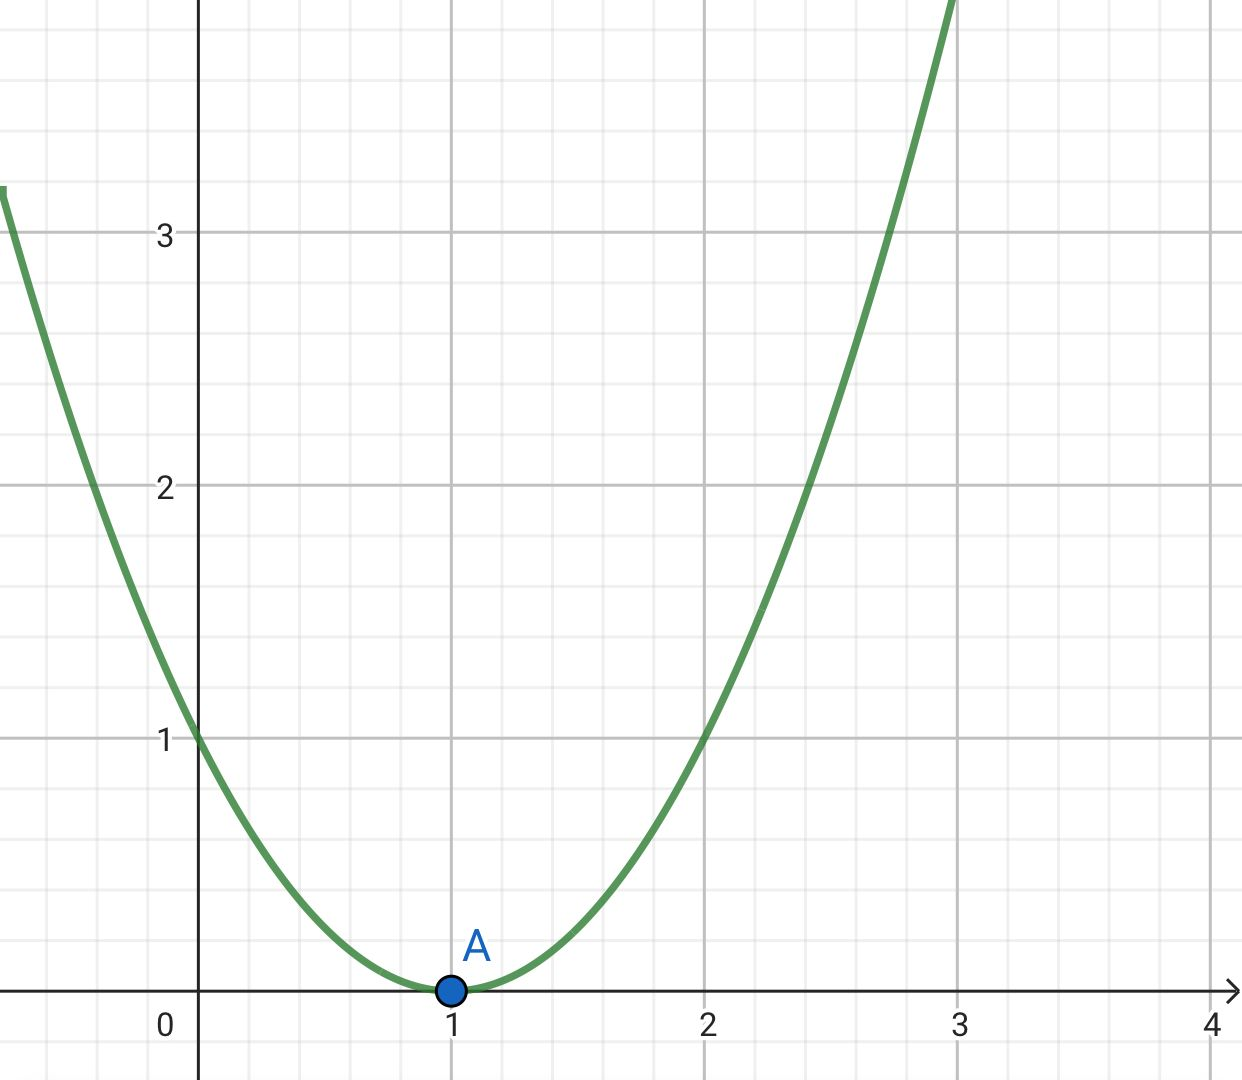
\includegraphics[height=8cm]{casoA.jpeg}
    \caption{Asociada a $(t-1)^2$}
    \label{fig:casoA}
\end{figure}\\
(b) velocidad cero y aceleración negativa;\\
\begin{figure}[h]
    \centering
    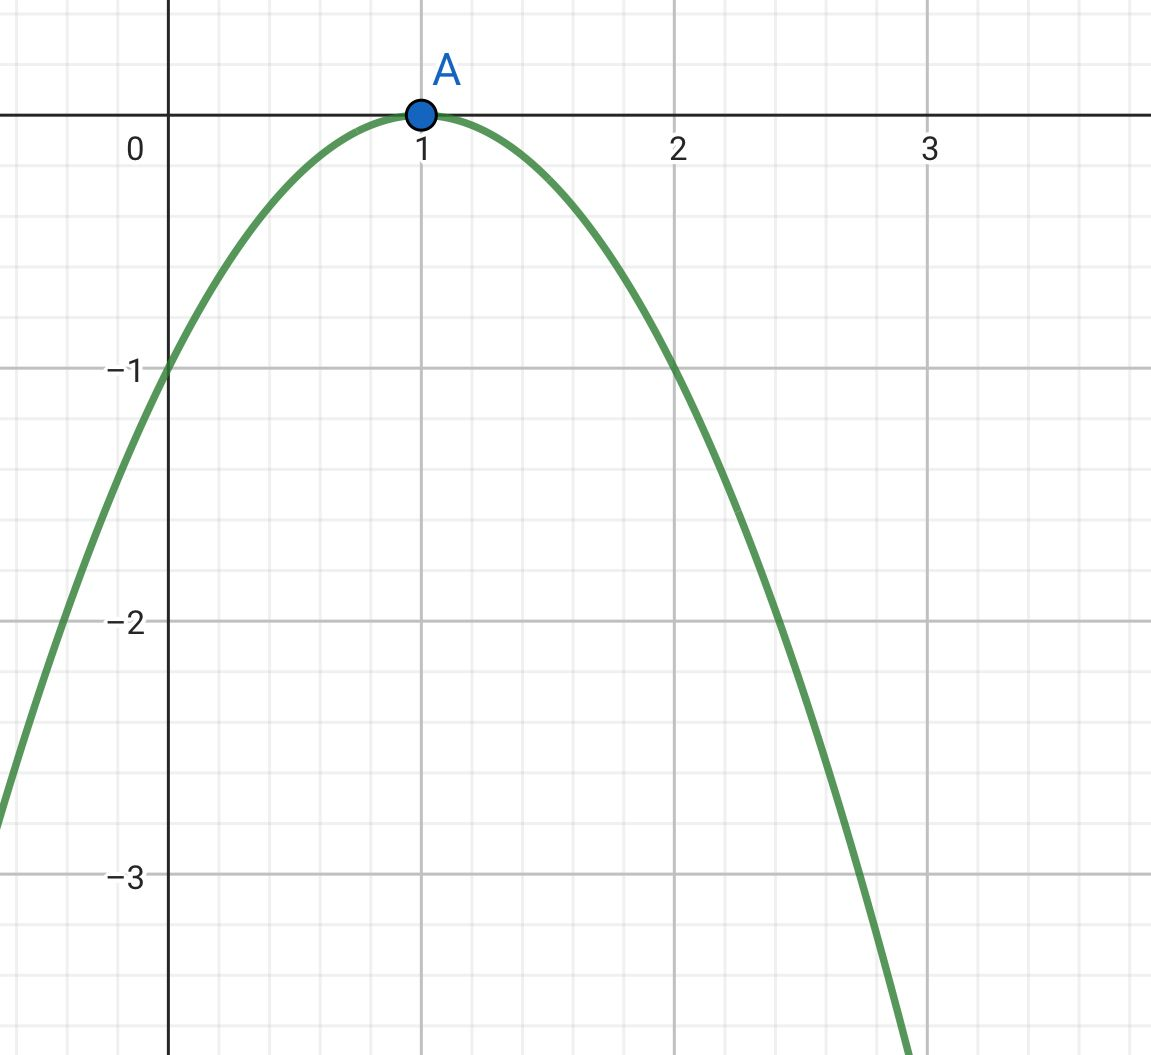
\includegraphics[height=8cm]{casoB.jpeg}
    \caption{Asociada a $-(t-1)^2$}
    \label{fig:casoA}
\end{figure}\\
 \newpage
(c) velocidad negativa y aceleración positiva;\\
\begin{figure}[h]
    \centering
    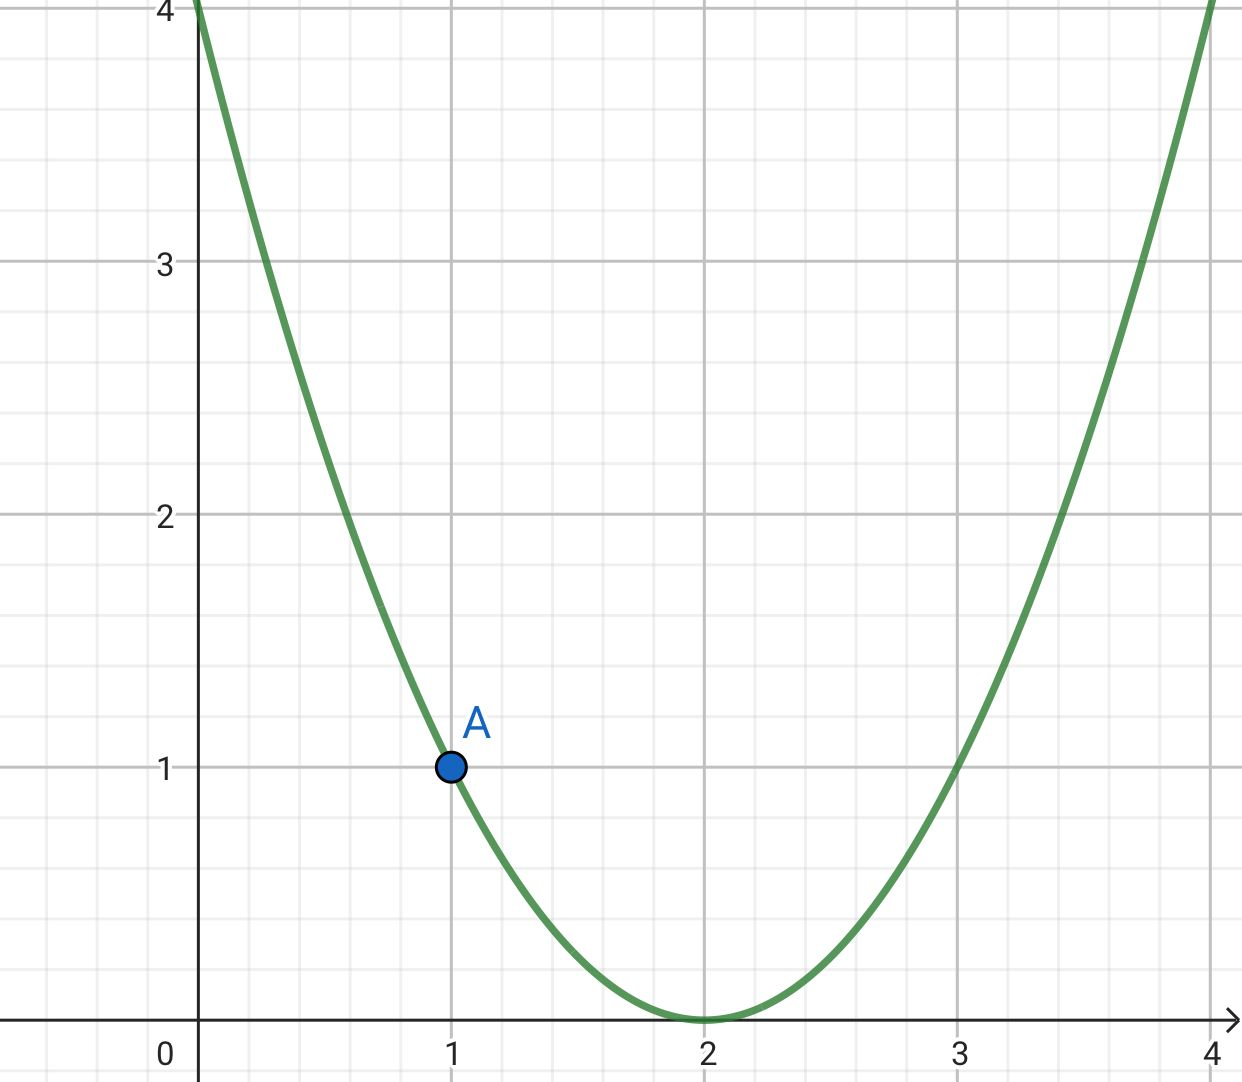
\includegraphics[height=8cm]{casoC.jpeg}
    \caption{Asociada a $(t-2)^2$}
    \label{fig:casoA}
\end{figure}\\
(d) velocidad negativa y aceleración negativa;\\
\begin{figure}[h]
    \centering
    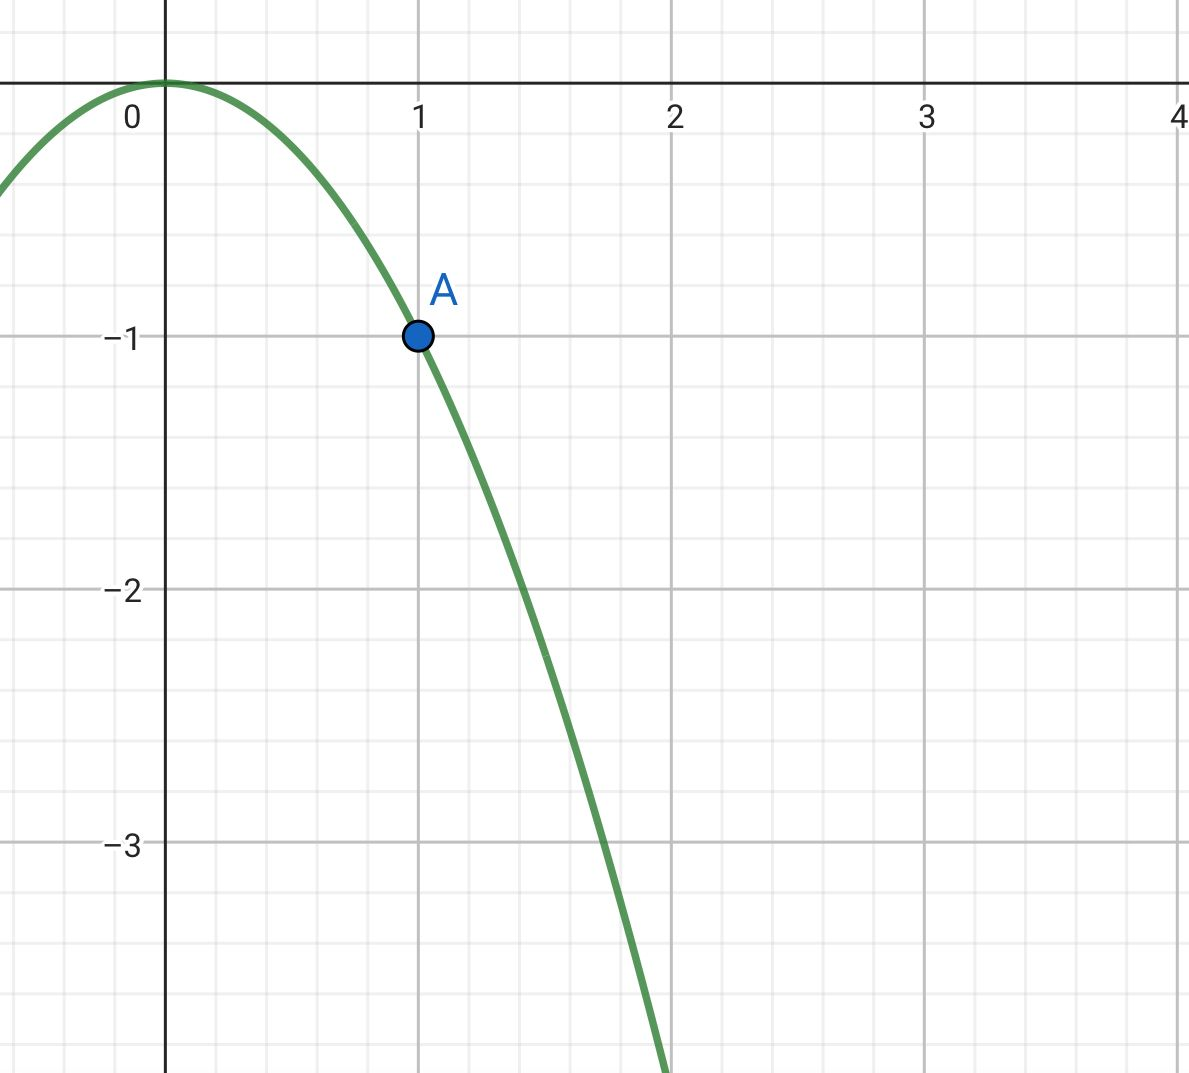
\includegraphics[height=8cm]{casoD.jpeg}
    \caption{Asociada a $-t^2$}
    \label{fig:casoA}
\end{figure}\\
(e) ¿En cuál de estas situaciones aumentará la velocidad de esta partícula en t = 1 s ?\\
\textit{Por la construcción de estas gráficas claramente se ve que a) y c), la diferencia en las rectas tangentes entre f(t) cuando t=1 -> t=2 crea un incremento en la pendiente, esto físicamente es la velocidad y la varianza positiva en las pendientes indica un aumento en su velocidad, que a su vez está directamente relacionado con el aumento de la aceleración; el intervalo entre t=1 y t=2 es muy grande por lo que tómese $\lim_{\Delta h -> 0} \Delta h$, aquí también incrementará la velocidad. Otra forma es usando la derivada de segundo orden de la posición x(t) en función del tiempo que nos proporciona la aceleración, esta en las funciones a) y c) es igual a 2 tal que este valor es una constante mayor que cero, esto indica que la velocidad incrementa a diferencia de b) y d) donde su derivada de segundo orden arroja a(t) = -2 < 0.}\\\\

\newpage
XXVI. La posición de una partícula a lo largo del eje x depende del tiempo de acuerdo con la ecuación:

\[x(t) = Ct^2 - Bt^3\]

\noindent Donde \(x\) está en metros y \(t\) en segundos.

\begin{enumerate}
  \item ¿Qué unidades SI deberán tener A y B? Para lo siguiente, haga que sus valores numéricos en unidades SI sean 3 y 1, respectivamente.
  \[
  [C][s^2] = [m] \Rightarrow [C] =  \frac{[m]}{[s^2]} \textit{  por otro lado B...  }
  [B][s^3] = [m] \Rightarrow [B] =  \frac{[m]}{[s^3]}
  \]
  \textit{Un método mucho más fácil es con la derivada de segundo y tercer orden, en donde C corresponde a unidades de aceleración y B al ser el único \textbf{"sobreviviente"} en j(t) corresponde a unidades de jerk.}
  
  \item ¿En qué tiempo llegará la partícula a su posición x positiva máxima? \\
  \[  x(t) = 3t^2 - t^3 \Rightarrow v(t) = \dot{x}(t) = 6t - 3t^2  \]
  \[ \textit{Puntos de pendiente 0:} \]
  \[ 3t (2-t) = 0 \therefore t_1 = 0 \cap t_2 = 2 \]
  \[ \textit{Máximos y mínimos:} \]
  \[ \ddot{x}(t) = 6 - 6t \]
  \[ \ddot{x}(0) = 6 \textit{  (Mínimo)  } \cap \textit{  }\ddot{x}(2) = -6 \textit{  (Máximo)  } \]
  \[ x(2) = 3(2)^2 - (2)^3 = 4m \]
  \[ \therefore \textit{La partícula alcanza su pósición máxima de 4m después de 2 segundos} \]
  
  
  \item ¿Qué longitud de trayectoria cubre la partícula en los primeros 4 s? ¿Cuál es su desplazamiento durante los primeros 4 s?\\
  \textit{La distancia la calculamos con la diferencia de posiciónes x(4) - x(0):}
  \[x(0) = 3(0)^2 - (0)^3 = 0\]
  \[x(4) = 3(4)^2 - (4)^3 = -16\]
  \[Distancia = |x_4-x_0| = |-16 - 0| = 16\]
  \textit{El desplazamiento con la suma de distancias en puntos importantes de la gráfica:}
  \[  Desplazamiento = \Delta x = x_4 - x_0 \Rightarrow -16 - 0 = -16m  \]
  \item ¿Cuál es la velocidad de la partícula al final de cada uno de los primeros cuatro segundos? ¿Cuál es la aceleración de la partícula al final de cada uno de los primeros cuatro segundos?

\begin{center}
\(
v(x) = \dot{x}(t) = 6t - 3t^2 \Rightarrow a(x) = \ddot{x}(t) = 6 - 6t\\
\)
  \begin{tabular}{|c|c|c|c|}
    \hline
    Tiempo (\(t\)) & Velocidad (\(v(t)\)) & Aceleración (\(a(t)\)) \\
    \hline
    1.0 & 3 & 6 \\
    2.0 & 0 & 0 \\
    3.0 & -9 & -6 \\
    4.0 & -24 & -12 \\
    \hline
  \end{tabular}
\end{center}

\item ¿Cuál es la velocidad promedio en el intervalo de tiempo de t = 2 a t = 4 s?\\
\begin{align*}
    v_{prom} &= n^{-1} \sum_{i=1}^n v_i \frac{m}{s}\\
    &= 2^{-1} \cdot (-24 - 0) \frac{m}{s}\\
    &= -12 \frac{m}{s}
\end{align*}
\end{enumerate}
\newpage

En el instante en que un semáforo cambia a luz verde, un automóvil arranca con una aceleración constante de 2.2 $ms^{-1}$. En el mismo instante un camión, que viaja a una velocidad constante de 9.5 $ms^{-1}$, alcanza y pasa al automóvil, (a) ¿A qué distancia del punto de arranque el automóvil alcanzaría al camión? (b) ¿A qué velocidad está viajando el automóvil en ese instante? (Es instructivo trazar una gráfica cualitativa de x contra t para cada vehículo.)\\
\textit{Considérese el mismo $\Delta x$ pues recorren la misma distancia.}
$$ v_{oA}t + 2^{-1}a_At^2 = 2^{-1}a_At^2 = \Delta x = v_{0C}t = v_{oC}t + 2^{-1}a_Ct^2$$
\begin{align*}
    \implies 2^{-1}a_At^2 &= v_{0C}t \\
    2^{-1}a_At^2 - v_{0C}t &= 0 \\
    t(2^{-1}a_At - v_{0C}) &= 0 \\
    2^{-1}a_At - v_{0C} &= 0 \\
    t &= \frac{2v_{0C}}{a_A} \\
    t &= \frac{2[9.5 \frac{m}{s}]}{2.2 \frac{m}{s^2}} \\
    t &\approx 8.63636 s
\end{align*}
\textit{Calcúlese ahora cuanto recorrió para alcanzar el camión (a).}
\begin{align*}
    v_{0c}t &= 9.5\frac{m}{s} \cdot \frac{2[9.5 \frac{m}{s}]}{2.2 \frac{m}{s^2}} \\
    v_{0c}t &\approx 82.0455m
\end{align*}
\textit{Ahora la velocidad en ese instante (b).}
\begin{align*}
    v_{fA} &= v_{0A} + a_At \\
    v_{fA} &= a_At \\
    v_{fA} &= [2.2 \frac{m}{s^2}]\left[\frac{2[9.5 \frac{m}{s}]}{2.2 \frac{m}{s^2}} \right] \\
    v_{fA} &= 19 \frac{m}{s}
\end{align*}

Es instructivo trazar una gráfica cualitativa de x contra t para cada vehículo.
\textit{Para esto usaremos la ecuación de la cinemática que relaciona la posición en función del tiempo con las variables aceleración y velocidad.}
\begin{align*}
    x_{automovil}(t) &= v_{oA}t + 2^{-1}a_At^2 \\
    &= 2^{-1}a_At^2 \\
    &= 2^{-1}2.2t^2 
\end{align*}
\textit{Nótese que la velocidad inicial del carro es cero al igual que su posición por nuestro sistema coordenado.}
\begin{align*}
    x_{camión}(t) &= v_{oC}t + 2^{-1}a_Ct^2 \\
    &= v_{0C}t \\
    &= 9.5t
\end{align*}
\textit{Obsérvese que la velocidad del camión es constante por lo que una vez rebasado jamás podrá volver a cruzarse (teóricamente, claro).}
\newpage
\begin{figure}[h]
    \centering
    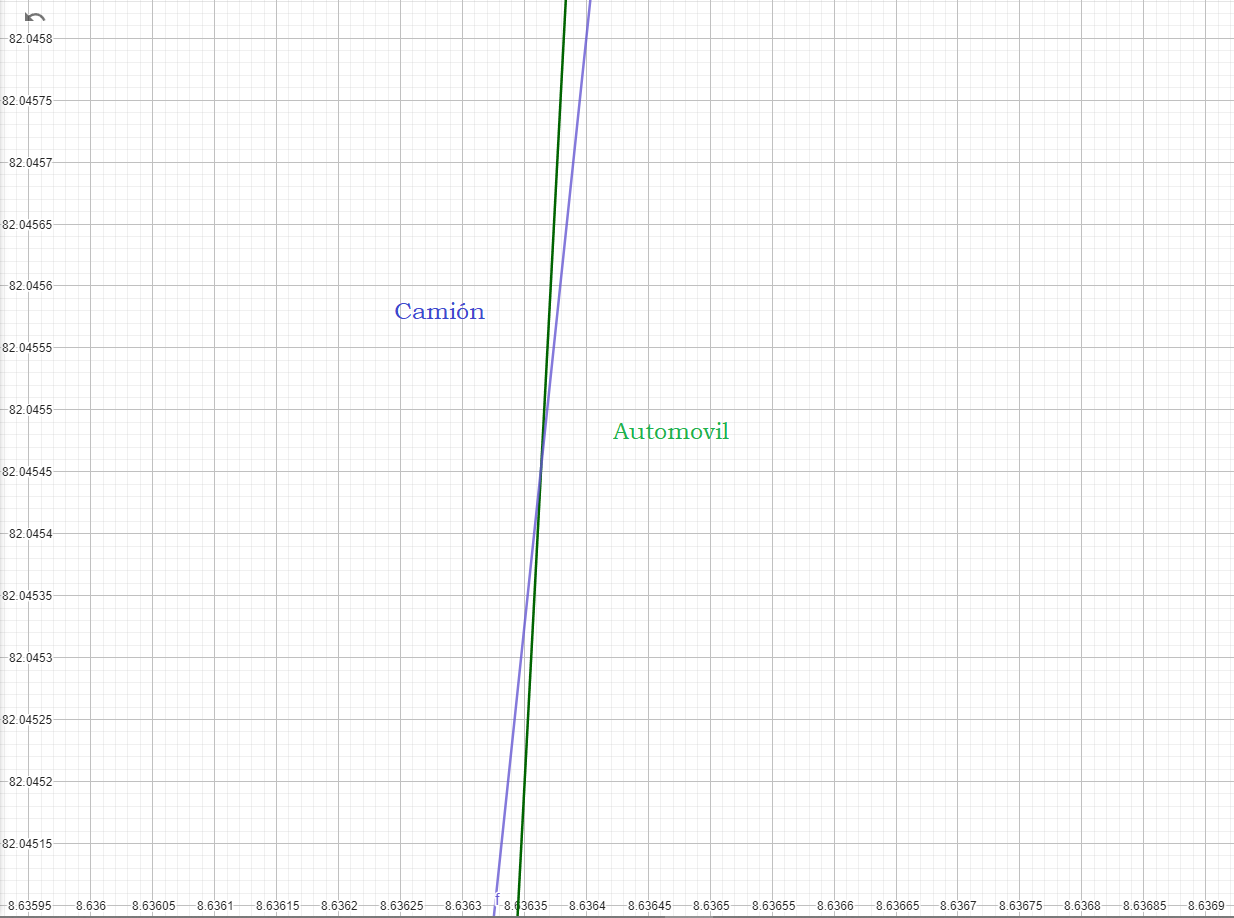
\includegraphics[height=10.5cm]{Camiona.png}
    \caption{Gráfica posición tiempo: Intersección automovil y camioneta}
    \label{fig:casoA}
\end{figure}\\
Mientras pensaba en Isaac Newton, una persona parada en un puente sobre una carretera deja caer inadvertidamente una manzana desde la barandilla justo cuando el extremo frontal de un camión pasa directamente abajo de la barandilla. Si el vehículo se está moviendo a 55 km/h (= 34 mi/h) y tiene una longitud de 12 m (= 39 ft), ¿qué tanto más arriba del camión deberá estar la barandilla si la manzana no logra golpear la parte trasera del camión?\\
\textit{Convertimos la velocidad del vehículo en metros sobre segundos a su vez que despejamos el tiempo que tarda en recorrer 12 segundos, obsérvese que la aceleración no existe.}
\begin{align*}
    t &= \frac{x}{v} \\
    &= \frac{12m}{55\frac{km}{h}\cdot \left[ \frac{\frac{m}{s}}{3.6\frac{km}{h}}\right]} \\
    &= \frac{12 \cdot 3.6 m}{55 \frac{m}{s}} \\
    &= \frac{43.2}{55}s \\
    &\approx 0.78545 s
\end{align*}
\textit{Dado que ya tenemos nuestro tiempo fijado, calcularemos el recorrido que haría la manzana en su componente y en aquel tiempo, véase que parte del reposo por lo que $v_0=0$ y su única aceleración es la gravitatoria}
\begin{align*}
    \Delta y &= v_{0y}t - \frac{gt^2}{2} \\
    &= - \frac{gt^2}{2} \\
    &\approx - \frac{9.806\frac{m}{s^2}\left[\frac{43.2}{55}s\right]^2}{2} \\
    &\approx -3.02485 m
\end{align*}
\textit{Véase que nuestro desplazamiento en y es negativo, esto geométricamente es correcto pues fijamos nuestro sistema coordenado tal que $\Vec{0}$ está justo en la manzana, entonces una caída representa un camino en el eje negativo de las y. Para ser más constructivos utilizareremos la magnitud de $\Delta y$ tal que esta adquirirá valor positivo.}\\
\textit{$\therefore$ La persona debe tirar \textbf{justo cuando el extremo frontal del camión pasa directamente abajo de la barandilla} a una altura de $3.02485 m$ por encima del camión para golpear la parte trasera.}}

\end{document}